
\documentclass{svproc}

\usepackage{url}
\def\UrlFont{\rmfamily}
\usepackage{natbib}%,bibspacing}
\usepackage{graphicx}
%\usepackage{subcaption}
\usepackage{bm}
%\usepackage{geometry}
\usepackage{float}
\usepackage{caption}
\usepackage{pdfpages}
\usepackage{setspace}
\usepackage{amsmath}
\usepackage{amssymb}
\usepackage{multicol}
\usepackage{color}
\doublespacing
\usepackage[margin=1in]{geometry}% to typeset URLs, URIs, and DOIs
\usepackage{url}
\def\UrlFont{\rmfamily}
\usepackage{biblatex}
\addbibresource{final_project.bib}

\begin{document}
\mainmatter              % start of a contribution
%
\title{Predicting Box Office Revenue}
%
\titlerunning{Box Office Revenue}  % abbreviated title(for running head)
%                                     also used for the TOC unless
%                                     \toctitle is used
%
\author{Jacob Merrell}
\institute{}
%
%%%% list of authors for the TOC(use if author list has to be modified)

\maketitle              % typeset the title of the contribution

\begin{abstract}
This study focuses on using random forests to predict movie box office revenue. The analysis reviews methods to collect the data, which variables have an impact on movie revenues, and irregularities in the data. Data simulations explore the bias and RMSE to determine how well similar data can be fit using random forests. Bootstrapping is used to measure the predictive power of the model. Issues not addressed in the paper and methods for improvement for future research are suggested. 
\end{abstract}

\section{Introduction}

Movies have been an integral part of society for nearly 100 years. Over the last 20 years consumers in the United States have spent more than \$10 billion per year to watch movies on the big screen \cite{The Numbers}. There is a lot of money to be made in the film industry. However, several films are financial liabilities to the studios that produce them. This study aims to predict how much money movies will gross at the box office. The ability to predict box office success is valuable to not only movie producing studios, but to investors as well. Accurate predictions of box office grosses help investors formulate expectations, and aid movie producers make decisions about which movies should and should not be made.

Before formulating predictions, we will address the methods and issues for data collection, and provide the statistical model used for prediction. Next, simulation studies will test the fit of the selected model, and lastly we will explore improvements to be made for future predictive models.

\newpage
\section{Data}

\subsection{Data Collection} 

All of the data used in this study was collected from The Numbers website. The Numbers was created in 1997 by Bruce Nash, and includes data for movies, actors/actresses, movie producing studios, release dates and more. A python script was created to collect the data. The numbers offers a report builder which allows users to input movie criteria and generate a list of at most 100 movies meeting the criteria. The python script looped through all possible months for all years of data offered by The Numbers, thus creating an exhaustive dataset of movies.

The following table shows the explanatory variables gathered from the website, and shows the class, and a brief explanation for each of the variables.

\begin{table}[ht]
\centering
\begin{tabular}{llll}
  \hline
 Name & Class & Explanation \\ 
  \hline
date & date & date of premier \\ 
  movie & character & movie name \\ 
  studio & factor & studio that produced movie \\ 
  genre & factor & genre of movie \\ 
  basedon & factor & what the story is based on \\ 
  actionanim & factor & live action or animated \\ 
  factfict & factor & factual or fictional \\ 
   budget & integer & cost to make \\ 
  thrcount & integer & how many theaters it opened in \\ 
   infdomgross & integer & inflation adjusted revenue \\ 
   direct & character & director \\ 
   compose & character & composer \\ 
   rating & factor & MPAA rating \\ 
   franch & character & which franchise \\ 
   actx & character & the xth actor listed in the movie \\ 
   \hline
\end{tabular}
\end{table}


There are 12,737 rows of data in this dataset associated with the above mentioned variables. Each row of data represent one movie.

\newpage
\subsection{Computed Data}

Analyzing box office grosses without adjusting for inflation is an apples to oranges comparison. All of the statistics calculated from the website's data are adjusted for inflation; that is all continuous statistics measured in dollars are inflation adjusted. We thought having a way to quantify popularity and past success would be crucial moving forward. In this study, the success and/or popularity of an actor, actress, movie studio, director, composer or franchise are all calculated by how much influence they have had in the recent past. We hypothesize that recent box office success (defined by a cumulative sum of box office gross over the previous 10 years) is a key indicator of popularity and overall success.

For example, Jim Carrey is a well-known actor whose fame reached its summit during the late 1990's. During the late 1980's however, Jim Carrey would not have been considered a superstar with nearly the same power to sell tickets. As he starred in movies that did well financially, his fame grew. However, fame is fickle, and an actor/actress's popularity fades. Since the late 1990's Jim Carrey has been involved in less box office hits. Even though his cumulative sum for box office gross is very high, he no longer enjoys high levels of popularity. As is the case for many actors, actresses, and directors, unless they are continually involved in blockbuster movies, their fame stagnates or declines. The following statistics were calculated from the original data, and aim to quantify popularity.

\begin{table}[ht]
\centering
\begin{tabular}{llr}
  \hline
 Name & Class & Explanation \\ 
  \hline
infbudget & integer & inflation adjusted cost to make movie \\ 
   avgfranchgross & integer & average revenue for all previous movies in franchise \\ 
  top1act & integer & cumulative career gross of the top actor (last 10 yrs) \\ 
   top3act & integer & cumulative career gross of the top 3 actors (last 10 yrs) \\ 
  top5act & integer & cumulative career gross of the top 5 actors (last 10 yrs) \\ 
  directgross & integer & cumulative career gross of director \\ 
  directgrosscur & integer & cumulative career gross of director (last 10 yrs) \\ 
   compgross & integer & cumulative career gross of composer \\ 
   compgrosscur & integer & cumulative career gross of composer (last 10 yrs) \\ 
   avgstudiogross & integer & cumulative career gross of studio \\ 
   avgstudiogrosscur & integer & cumulative career gross of studio (last 10 yrs) \\ 
   inffirstweeknd & integer & total domestic gross during the first weekend \\
   \hline
\end{tabular}
\setlength{\tabcolsep}{3em}
\end{table}

\newpage
\subsection{Exploratory Data Analysis}
With the statistics of interest and other explanatory variables in place, we examined the data to look for any irregularities. We noticed differences between inflation adjusted grosses before and after the year 2000, and also in inflation adjusted budgets. These differences are shown below.

\begin{center}
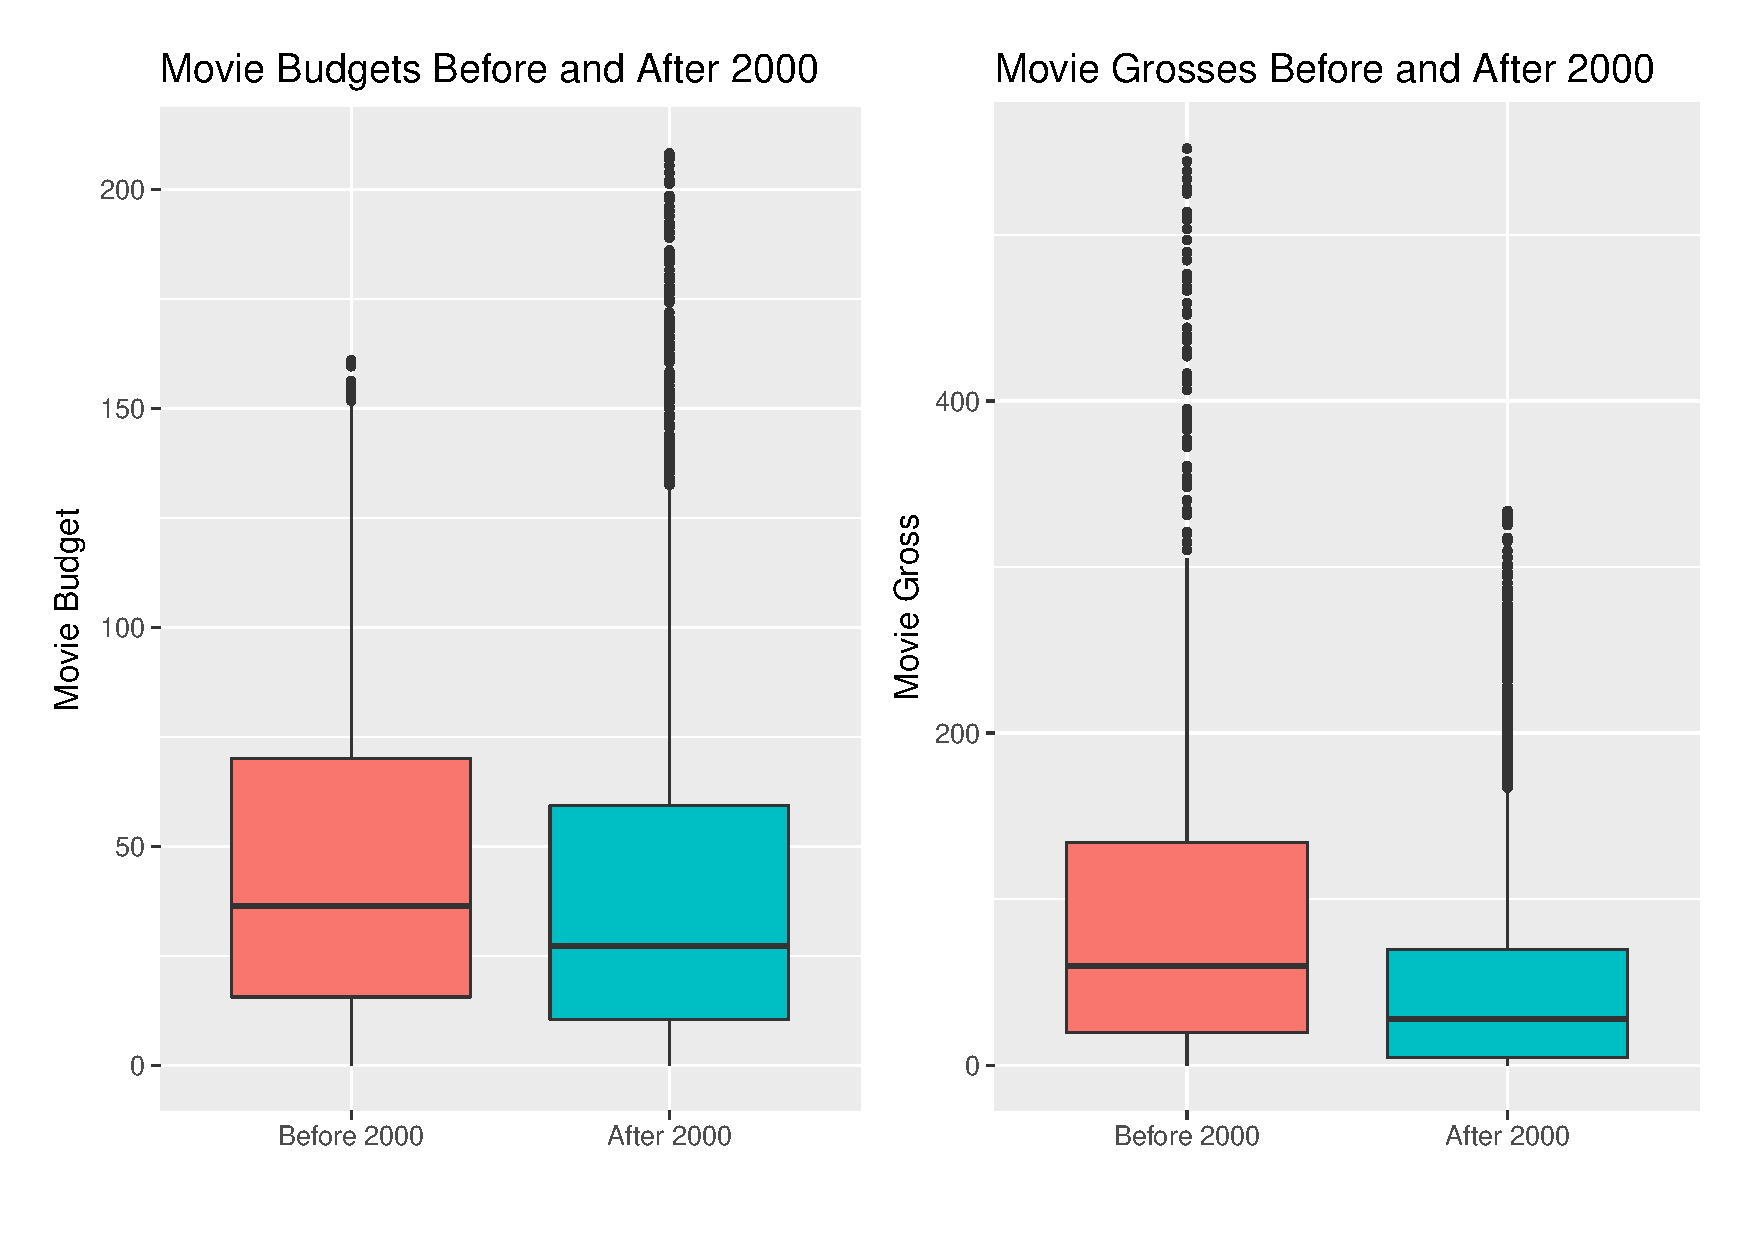
\includegraphics [height=8cm]{dataissue.pdf}
\end{center}

As seen in the chart above, movie budgets before and after 2000 have similar inner quartile ranges (IQR), however, movies made after 2000 have many more outliers. Few movies made before 2000 have very large budgets. This may be caused by technological advances and special effects. Newer movies are made with CGI, and costly special effects, therefore newer movie budgets are inflated. The box plot on the right shows movies before 2000 have more success in the box office. Not only is the IQR larger for older movies, but many of the outliers for inflation adjusted gross were of movies made before 2000. A logical explanation may be the way media is consumed currently. Many people have access to Netflix, Red Box, the internet, and other methods of watching movies. In the past, the options were limited. For example, a theater goer in 1930 would either have to see the movie in theaters, or never see the movie; internet, television, etc. were not available at the time.

Given the discrepancies in the data, we decided to limit the study to movies made after (and including) January 1st, 2000. This should give more reliable data as more recent history should reflect current trends better than older data. The new dataset had the same variables, but 2,344 rows.

\newpage
\section{Modeling}

\subsection{Random Forest}

The variable of interest in the study is inflation adjusted gross. Since the goal of the study is predicting box office revenue and not inference, random forests are used. Random Forest is a decision tree method that can be used for classification and regression. At each node, a set number of variables are randomly selected from the predictor variables. The variable that splits the data best is used. The cut-off value of the chosen predictor variable that best splits up the data is the criteria for placing the observations in groups. The process is repeated at each node, randomly selecting variables, and splitting the data until there is no clear separation. This is called a tree. Multiple trees are made, and the results of each tree are averaged to give more accurate classifications and predictions.


\subsection{Optimal Number of Trees}

Results are more accurate with a larger number of trees, but computational time could be drastically increased. For this study we want to know what is the smallest number of trees that will provide accurate results. The graph below helps answer that question. 

\begin{center}
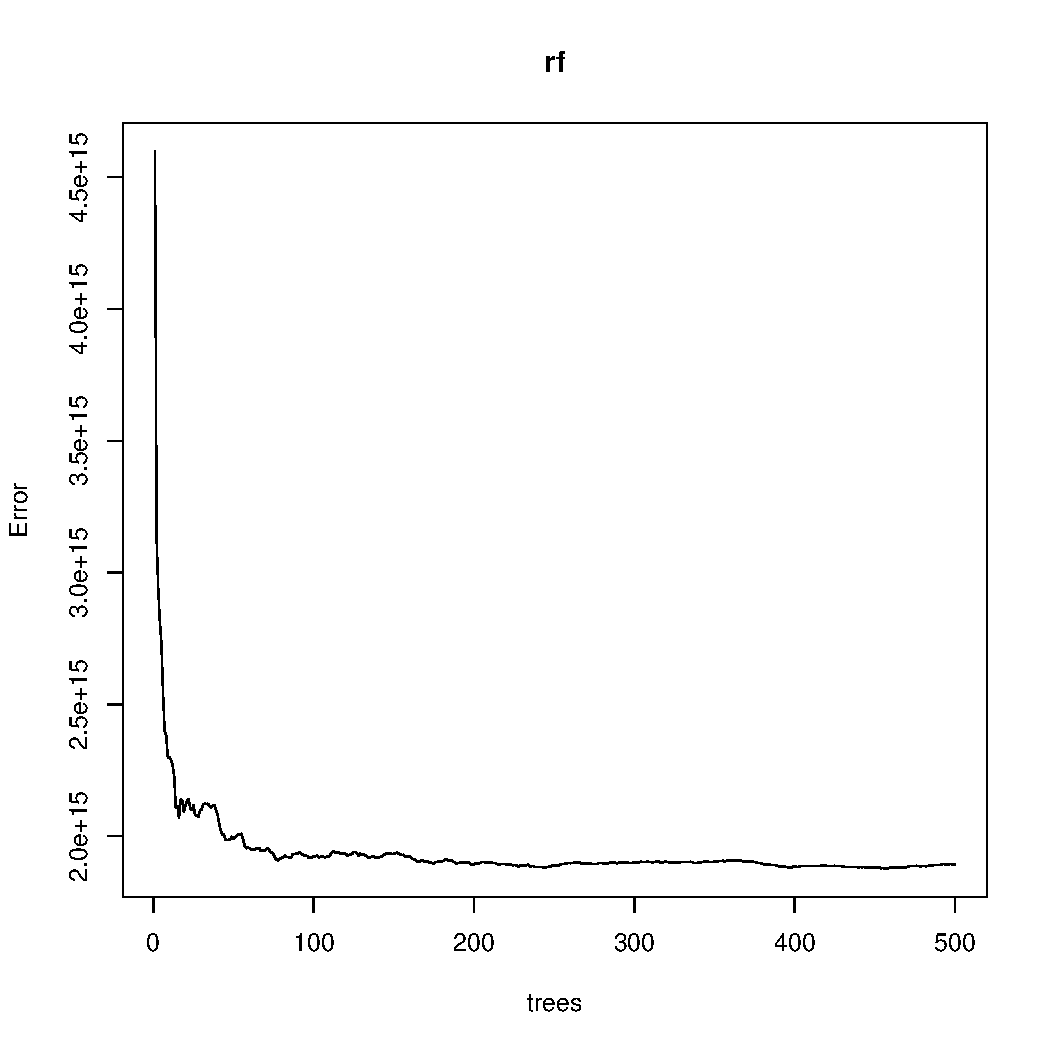
\includegraphics [height=8cm]{optim_trees.pdf}
\end{center}

For this we will use 100 as the number of trees, since it small enough that it won't slow down calculations, but it decreases the error drastically using 100 trees.

\subsection{Optimal Number of Variables}

At each node a random number of variables is selected for consideration. We iterate through all the posibilities (17 since there are 17 explanatory variables), to see which one provides the lowest error.

\begin{center}
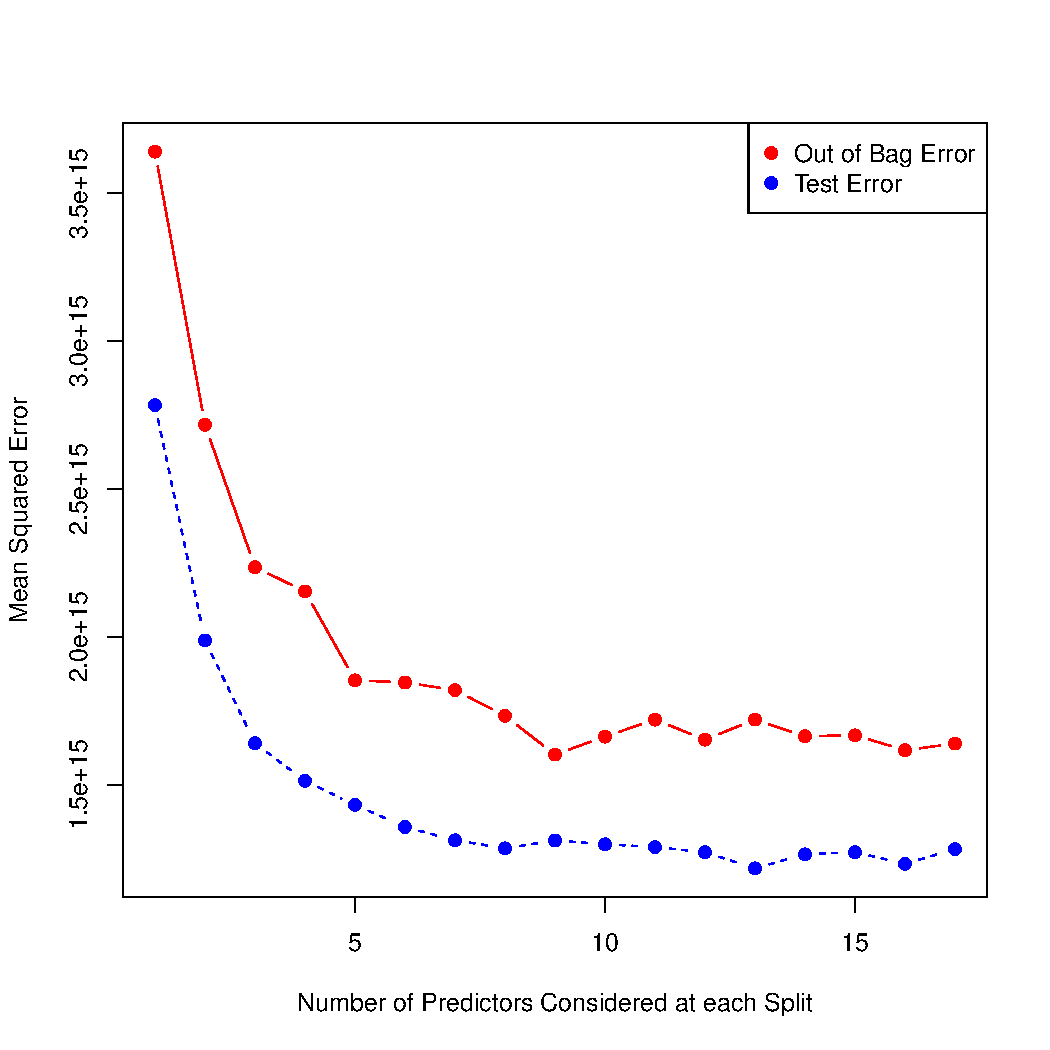
\includegraphics [height=8cm]{mtry.pdf}
\end{center}

The number of variables that should be used at each node is 9, because it provides the least amount of error.

\newpage
\section{Simulation Studies}

\subsection{R-Squared, Bias and RMSE}

Testing whether or not the random forest process is a good fit for the type of data we have can be done through simulation. After generating random data sets, we fit the same model as in the previous section to the newly generated data. With the fitted model, we calculate the R-squared, bias and RMSE by comparing the randomly generated inflation adjusted grosses to the predicted grosses from the model. This process was iterated 1,000 times to observe the distribution of the bias and RMSE.

\begin{center}
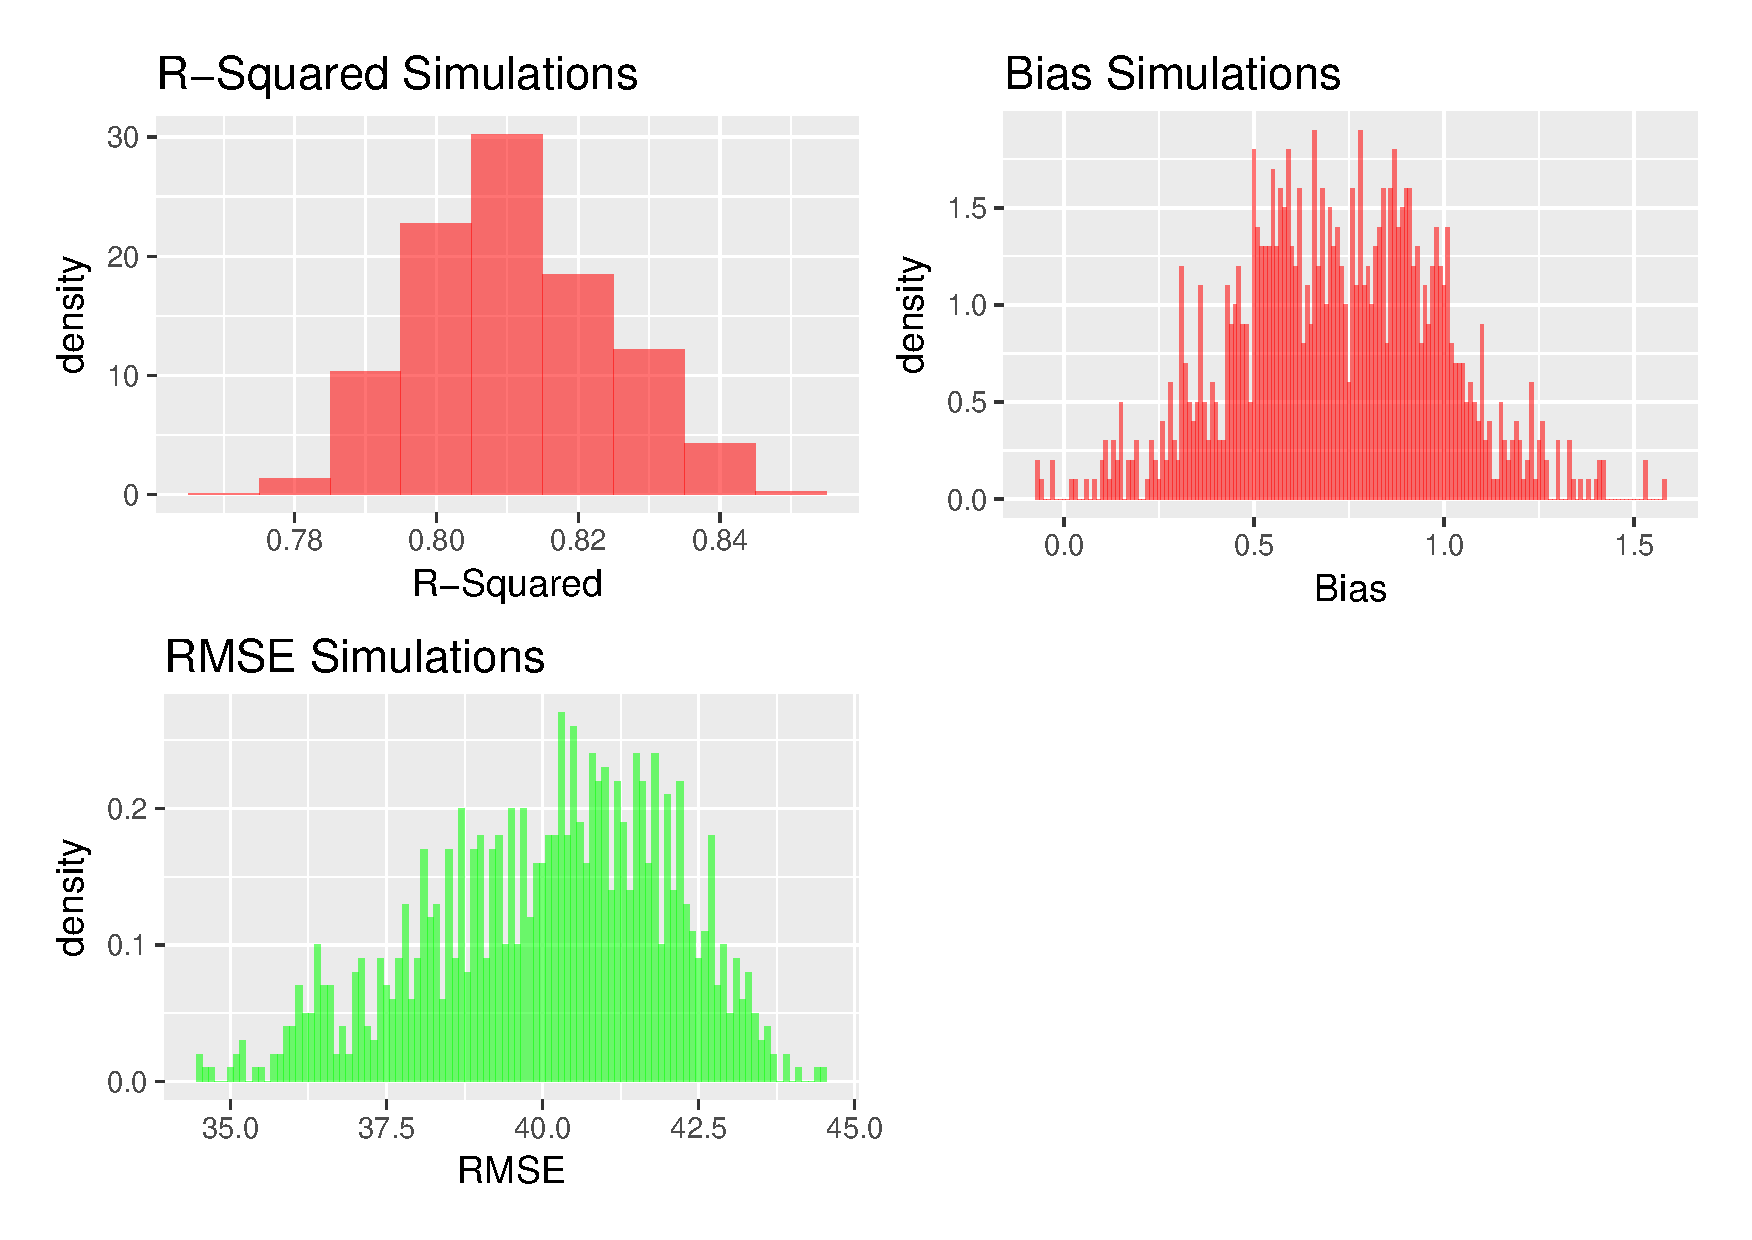
\includegraphics [height=8cm]{biasmse.pdf}
\end{center}

The R-squared values are high meaning the random forest accounts for most of the variation in box office revenue. The bias and RMSE in the histograms above are both displayed in millions of dollars. The bias is very small, and centered around 0. The RMSE penalizes response variables with large values since being off by even a small percentage can inflate the errors rapidly, since the errors are squared. The high RMSE may be a result of the model's tendency for conservative estimates; when there are outliers, which there are several, the predictions underestimate the actual values. The table below shows the average estimate and the average inflated adjusted gross for movies which made a large amount of money versus movies that only made an average amount of money at the box office.

\begin{table}[ht]
\centering
\begin{tabular}{rrr}
  \hline
 & Mean of Observed Values & Mean of Predicted Values \\ 
  \hline
Movies Above \$400 million & 509.04 & 388.13 \\ 
  Movies Between \$80 and \$120 million & 98.40 & 98.60 \\ 
   \hline
\end{tabular}
\end{table}

This shows that the model under estimates movies with high box office totals and verifies the hypothesis that the large RMSE values are caused in part by the model's under estimation of box office hits. Also as hypothesized for more average movie revenues, the model predicts much more accurately.

\section{Future Research}
The proposed model in this study made some fairly accurate predictions given the limited explanatory variables and time constraints. Here are suggestions we have for those wishing to further our research of box office revenue.

First, more explanatory variables should be explored. Some potential variables of interest might include Rotten Tomatoes scores, IMDb, or other critic/audience reviews. One of the reasons for excluding this type of data from the analysis was because of insignificant results from other research papers. However, many of these studies only included ratings as explanatory variables, and few other variables. Perhaps ratings were not significant in their models, but coupled with other explanatory variables there may be some significant interactions. Also, including data that quantifies consumer enthusiasm could be very predictive. For example including a variable that includes the number of Google searches for a movie before its release, or social media posts about the movie.

Also, transformations and interactions make the model more significant. With fewer time constraints transformations of the data and interactions could help explain more of the variation in the revue of box office hits. A distribution with thicker tails or more probability at the extremes could have also helped address the issue of under estimating high grossing movies.


\section{Conclusion}

There is a lot of money to made or lost in the movie industry. It is imperative for investors and movie producers to know what variables can influence box office grosses. The main goal of this study was to predict box office revenue, and the random forest model explained about 80 percent of the variation in box office revnue. Even the though the model predicted box office revenue fairly well, future studies and access to better data may lead to more accurate predictions of box office revenue.




\begin{thebibliography}{6}



\bibitem {The Numbers}
Nash Information Services, LLC: The Numbers.
(2017). \url{https://www.the-numbers.com/}

\bibitem{R}
R: A Language and Environment for Statistical Computing,R Core Team.R Foundation for Statistical Computing},
(2017). \url{https://www.R-project.org/}
  


\end{thebibliography}
\end{document}
